\section{Darstellung der Ergebnisse und Auswertung}

\subsection{Untersuchung des chaotischen Verhaltens}
Zunächst wurde das Pendel aus, soweit händisch möglich, gleichen Anfangsbedingungen gestartet. Der Startpunkt wurde hier mittels einer an einem der beiden Tische befestigten Gewindestange festgehalten. Das Pendel wurde dann in Ruhe so gestartet, dass sich die obere Masse($ m_{1} $) direkt neben der Gewindestange befand. Aufgrund dieser Anordnung kann ein geschätzter Fehler von $ 5  mm $ für den Ort der oberen Masse und dementsprechend auch für den Ort der unteren Masse angenommen werden.

\begin{figure}
        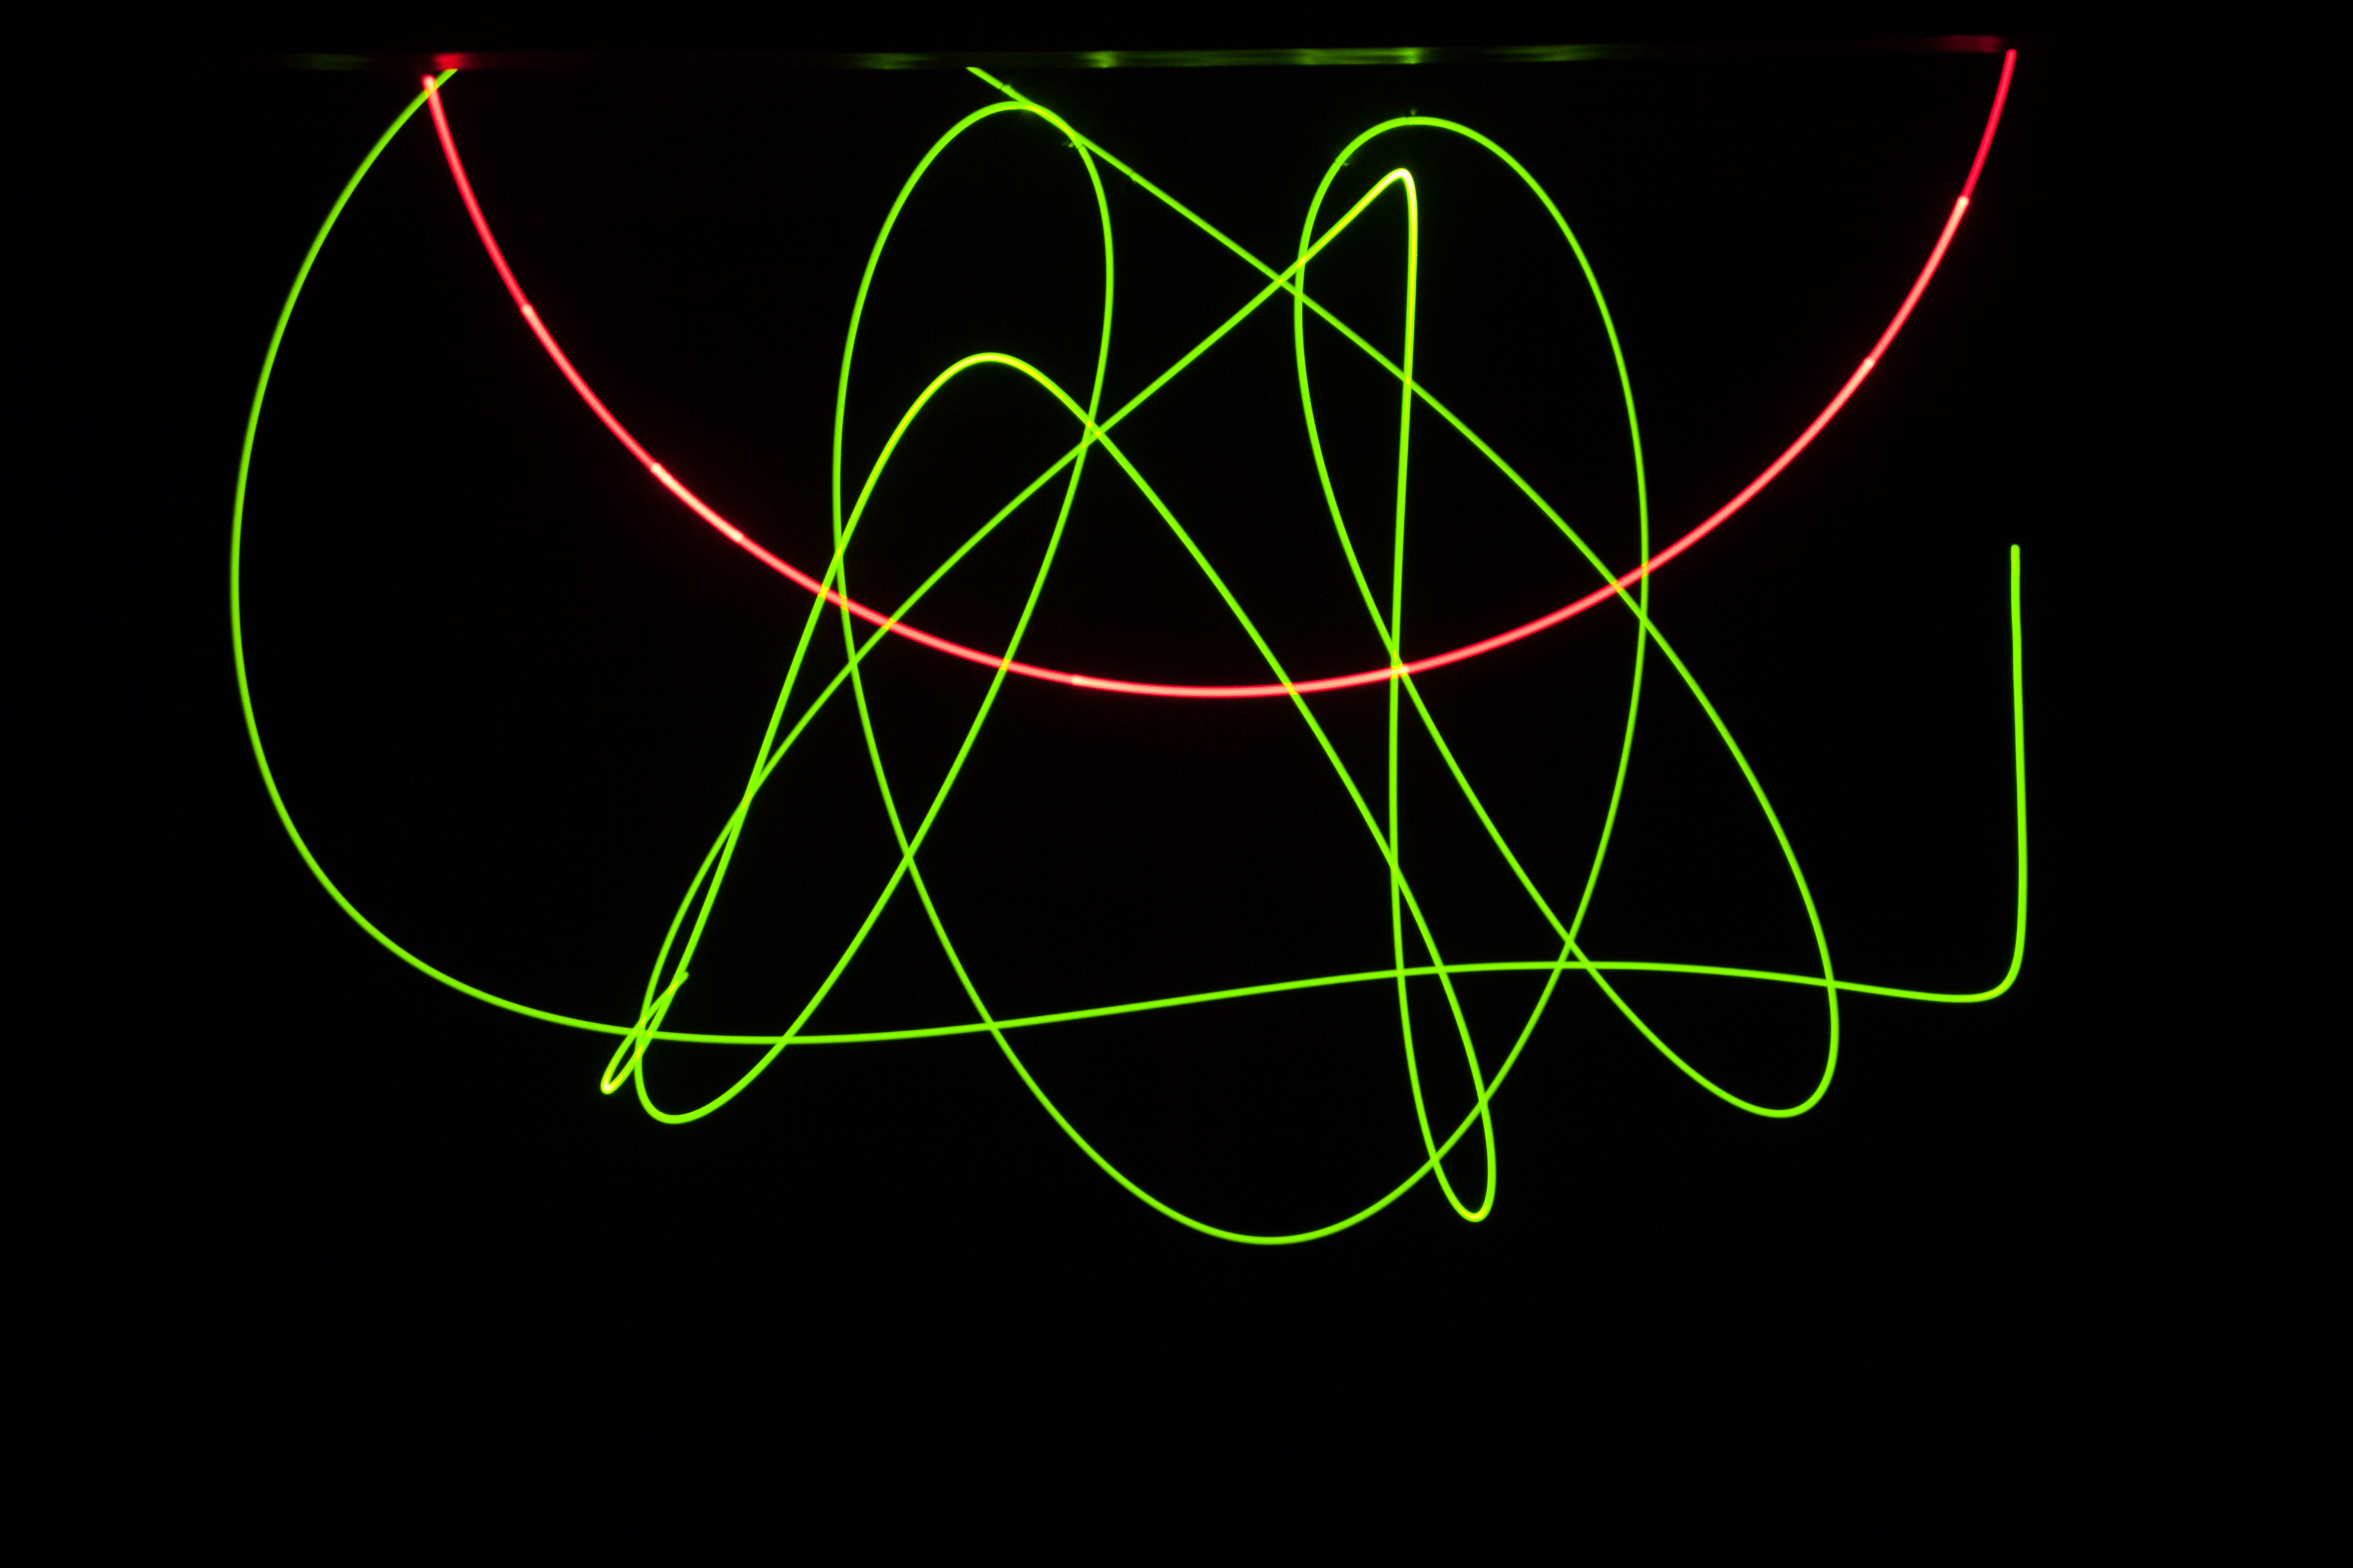
\includegraphics[width=.9\textwidth]{images/pendel-10.jpg}
\caption{2. Verlauf}
\label{pendel-10}
\end{figure}

\begin{figure}
        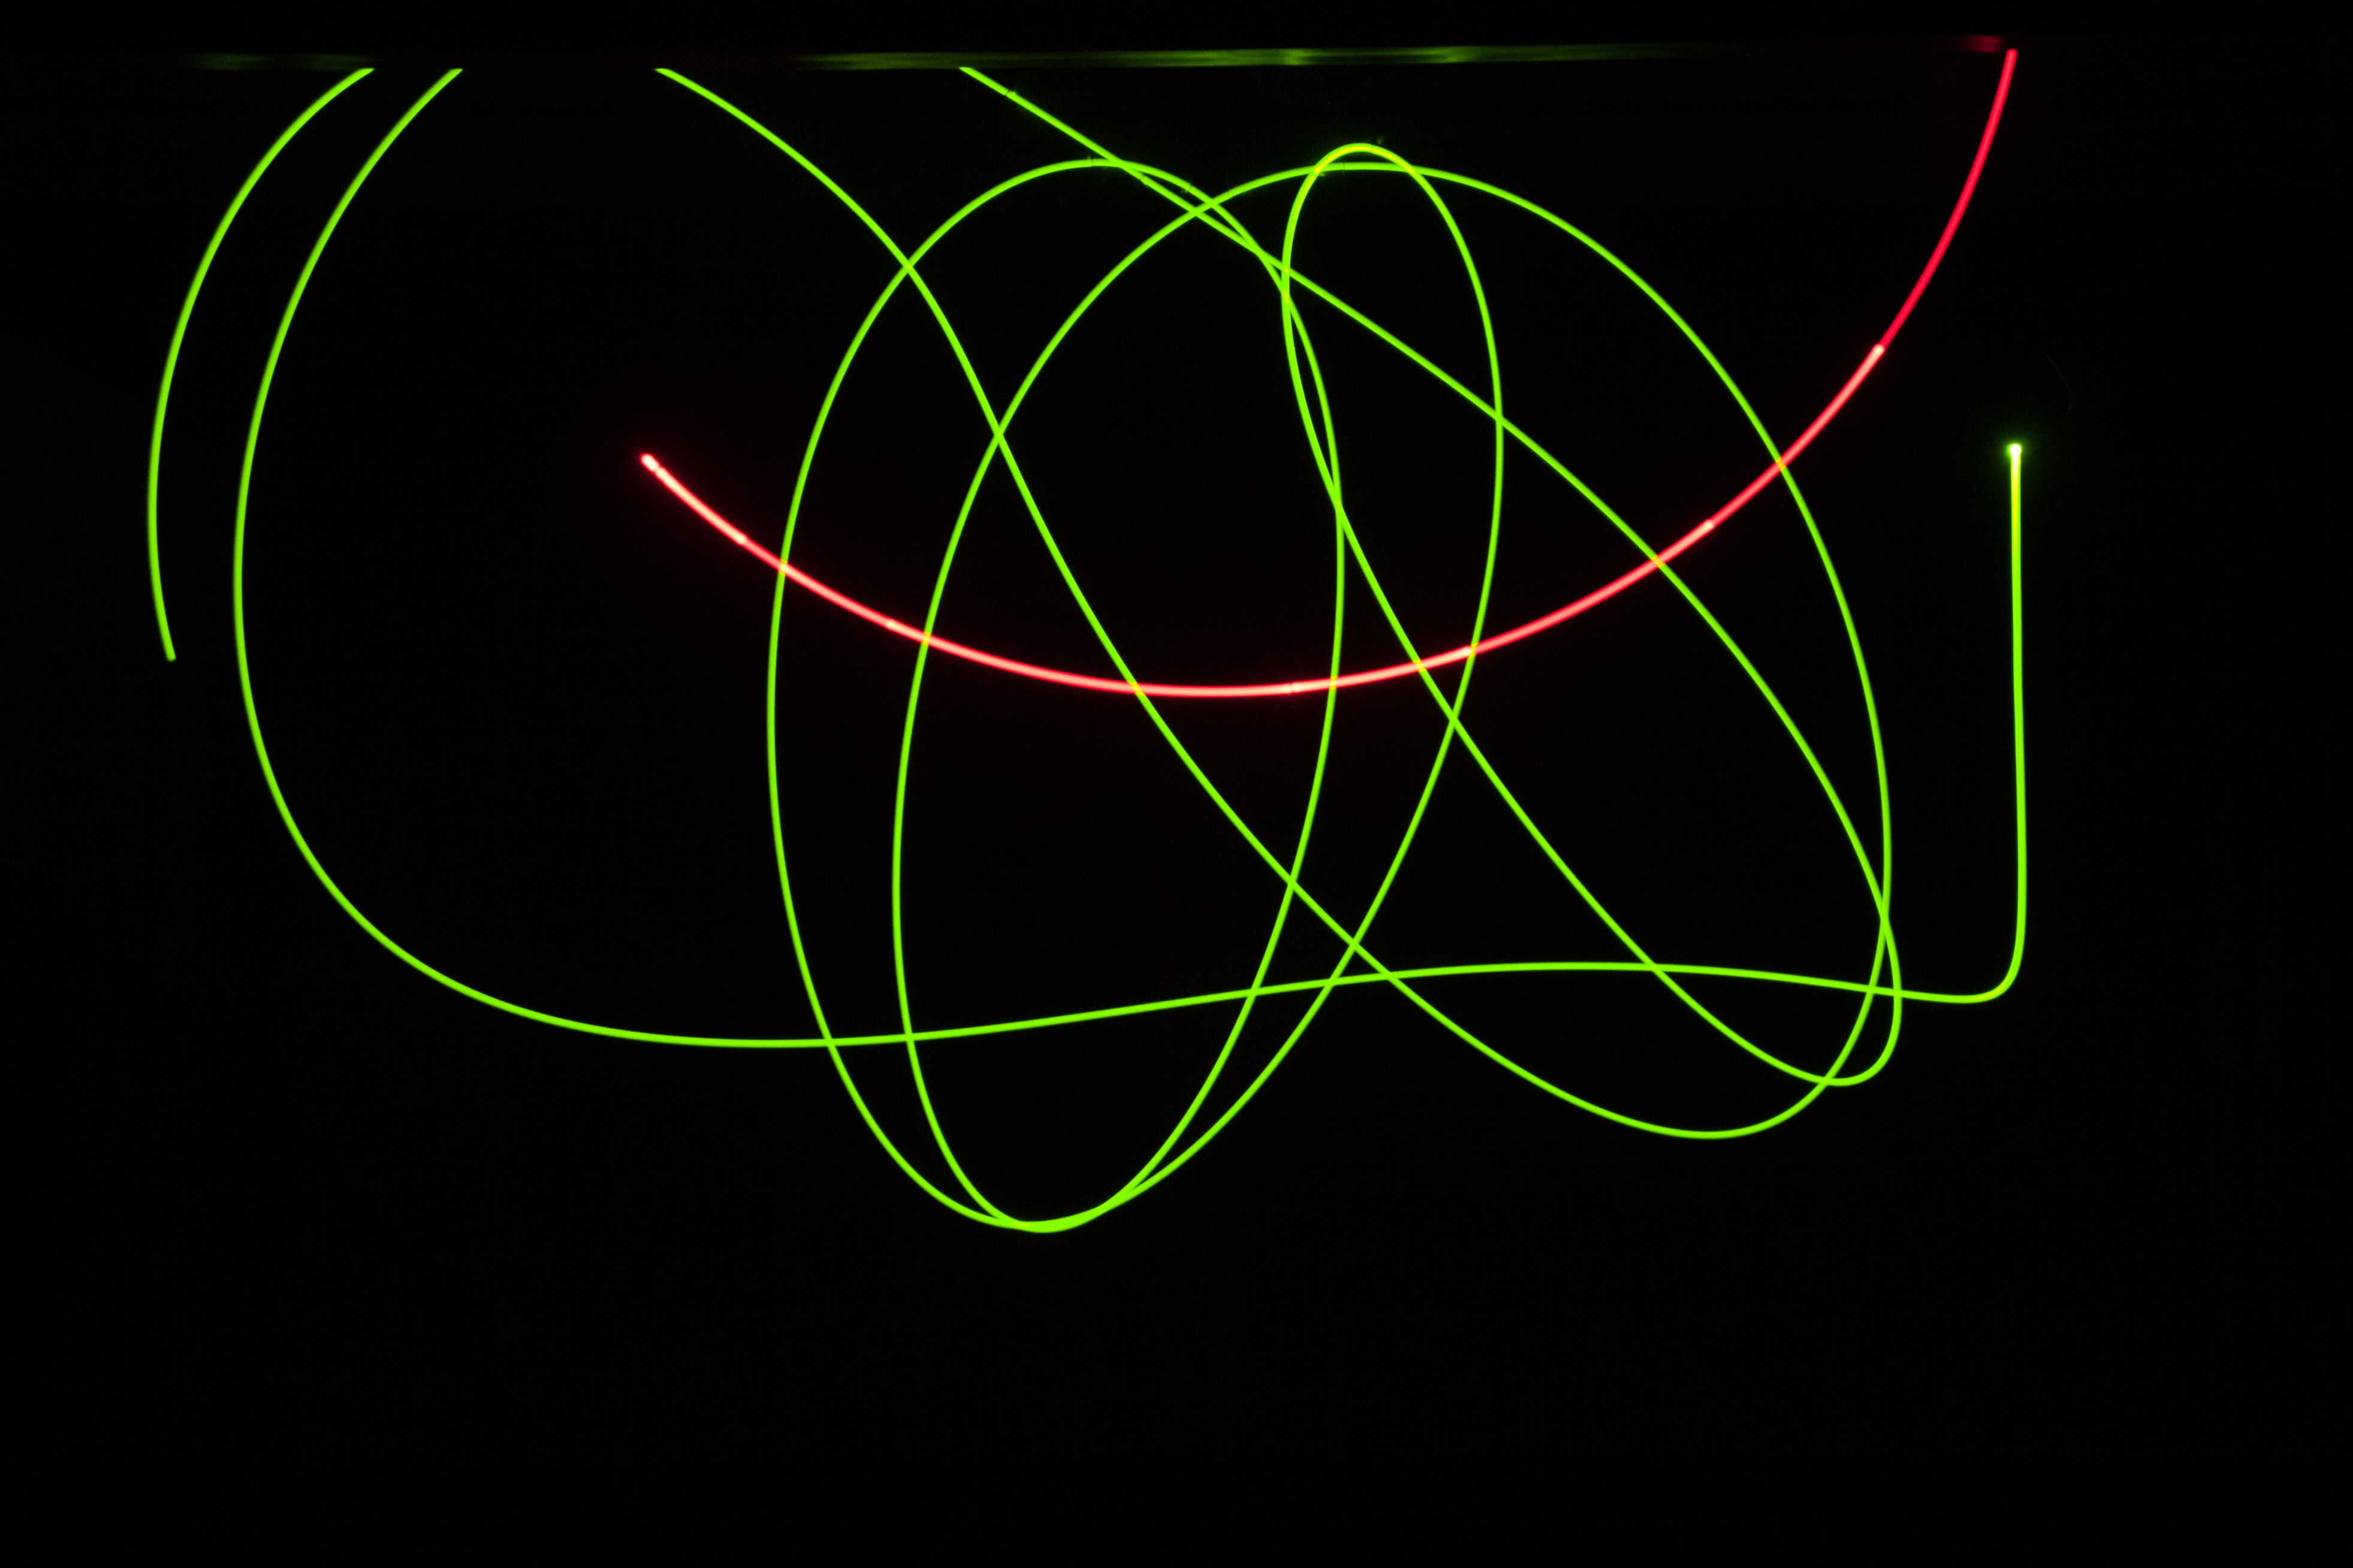
\includegraphics[width=.9\textwidth]{images/pendel-9}
\caption{3. Verlauf}
\label{pendel-9}
\end{figure}

Vergleicht man drei exemplarisch ausgewählte Aufnahmen (\ref{pendel-6}, \ref{pendel-10}, \ref{pendel-9}) (Belichtungszeit jeweils $3.2s$), so zeigt sich, dass der Verlauf der grünen Leuchtspur des unteren Pendels zumindest der groben Form nach gleich ist bis zu dem mit einem roten Pfeil markierten Punkt. Danach differierten die Wege der unteren Masse deutlich, bis nach etwa einer halben weiteren Schwingung überhaupt kein sichtbarer Zusammenhang mehr zwischen den Leuchtspuren besteht. Während in \ref{pendel-6} und \ref{pendel-9} die Spur von dem markierten Punkt ausgehend einen Bogen nach rechts beschreibt, wird in \ref{pendel-10} die untere Masse abgebremst, sodass sie, wie an der deutlich helleren Färbung der Leuchtspur zu erkennen, fast zum Stehen kommt und danach annähernd senkrecht nach unten weiterführt. Der Grund für die hellere Färbung bei langsameren Geschwindigkeiten und insbesondere Punkten, bei denen sich die Geschwindigkeitsrichtung umkehrt, ist, dass ein Punkt auf der Leuchtspur umso heller ist, je länger sich die an der Masse befestigte Diode im Abstand der halben Breite der Leuchtspur (des \enquote{optischen Radius} der Diode) von diesem Punkt befindet. 
Weiter divergiert auch der Verlauf von \ref{pendel-6} und \ref{pendel-9} bald, wie in den Abbildung gut zu erkennen ist. 
Dieses Verhalten entspricht dem in der Theorie dargestellten chaotischen Verhalten, sodass das Doppelpendel als ein chaotisches System bezeichnet werden kann. 

\subsection{Betrachtung der Reibung}

\subsubsection{Allgemeines zur Auswertung}
Gewählt wurde für die Auswertung ein Fall mit kleiner Auslenkung, weil die Messpunkte so durch numerische Berechnung in Näherung nachvollzogen werden konnten.
Für die Betrachtung der Reibung wurde ein Video aufgenommen und mittels eines Tracking-Programms nachträglich ausgewertet. 
Da aus den Tracking-Daten nur die einzelnen Koordinaten der Massepunkte hevor gehen, aber nicht die Koordinaten des Aufhänungspunktes des oberen Pendels, muss dieser noch separat ermittelt werden. Dies wurde mittels einer Berechnung in python erreicht, wobei ein Algorithmus implementiert wurde, der für jeden Punkt $(x, y)$ eines Rasters die Abstände $d_1, d_2, ... $ zu den Messpunkten des oberen Pendels $(x_1, y_1), (x_2, y_2), ...$ ermittelt und die stochastische Varianz dieser Abstände berechnet. Als Koordinatenursprung wird dann der Punkt mit minimaler Varianz des Abstandes verwendet, d.h. der Punkt, an dem die Abstände zu allem Messpunkten des oberen Pendels ungefähr gleich sind, sodass sich die \enquote{Länge} des ersten Pendels im Rahmen der Messgenauigkeit als konstant ergibt.  
Für die weitere Auswertung für jeden Zeitpunkt $ t $ einer Aufnahme die Geschwindigkeit von einem Massepunkt zu dieser Zeit mittels
\begin{equation}
\vec{v}(t) = \frac{1}{(2 \Delta t)} \cdot (\vec{x}(t+\Delta t) - \vec{x}(t-\Delta t))
\end{equation} 
berechnet. 
Somit verhindert man eine \enquote{Verschiebung} zwischen den Ortskoordinaten $  \vec{x} (t) $ und $ \vec{v} $ , die sich ergeben würde, wenn man nur das Intervall $ [t - \Delta t, t] $ betrachtet. Hier würde man einem Ort (und der damit verbundenen kinetischen Energie) eine \enquote{frühere} und damit falsche Geschwindigkeit zuordnen. 
\subsubsection{Betrachtung der Messergebnisse}


\begin{figure}
        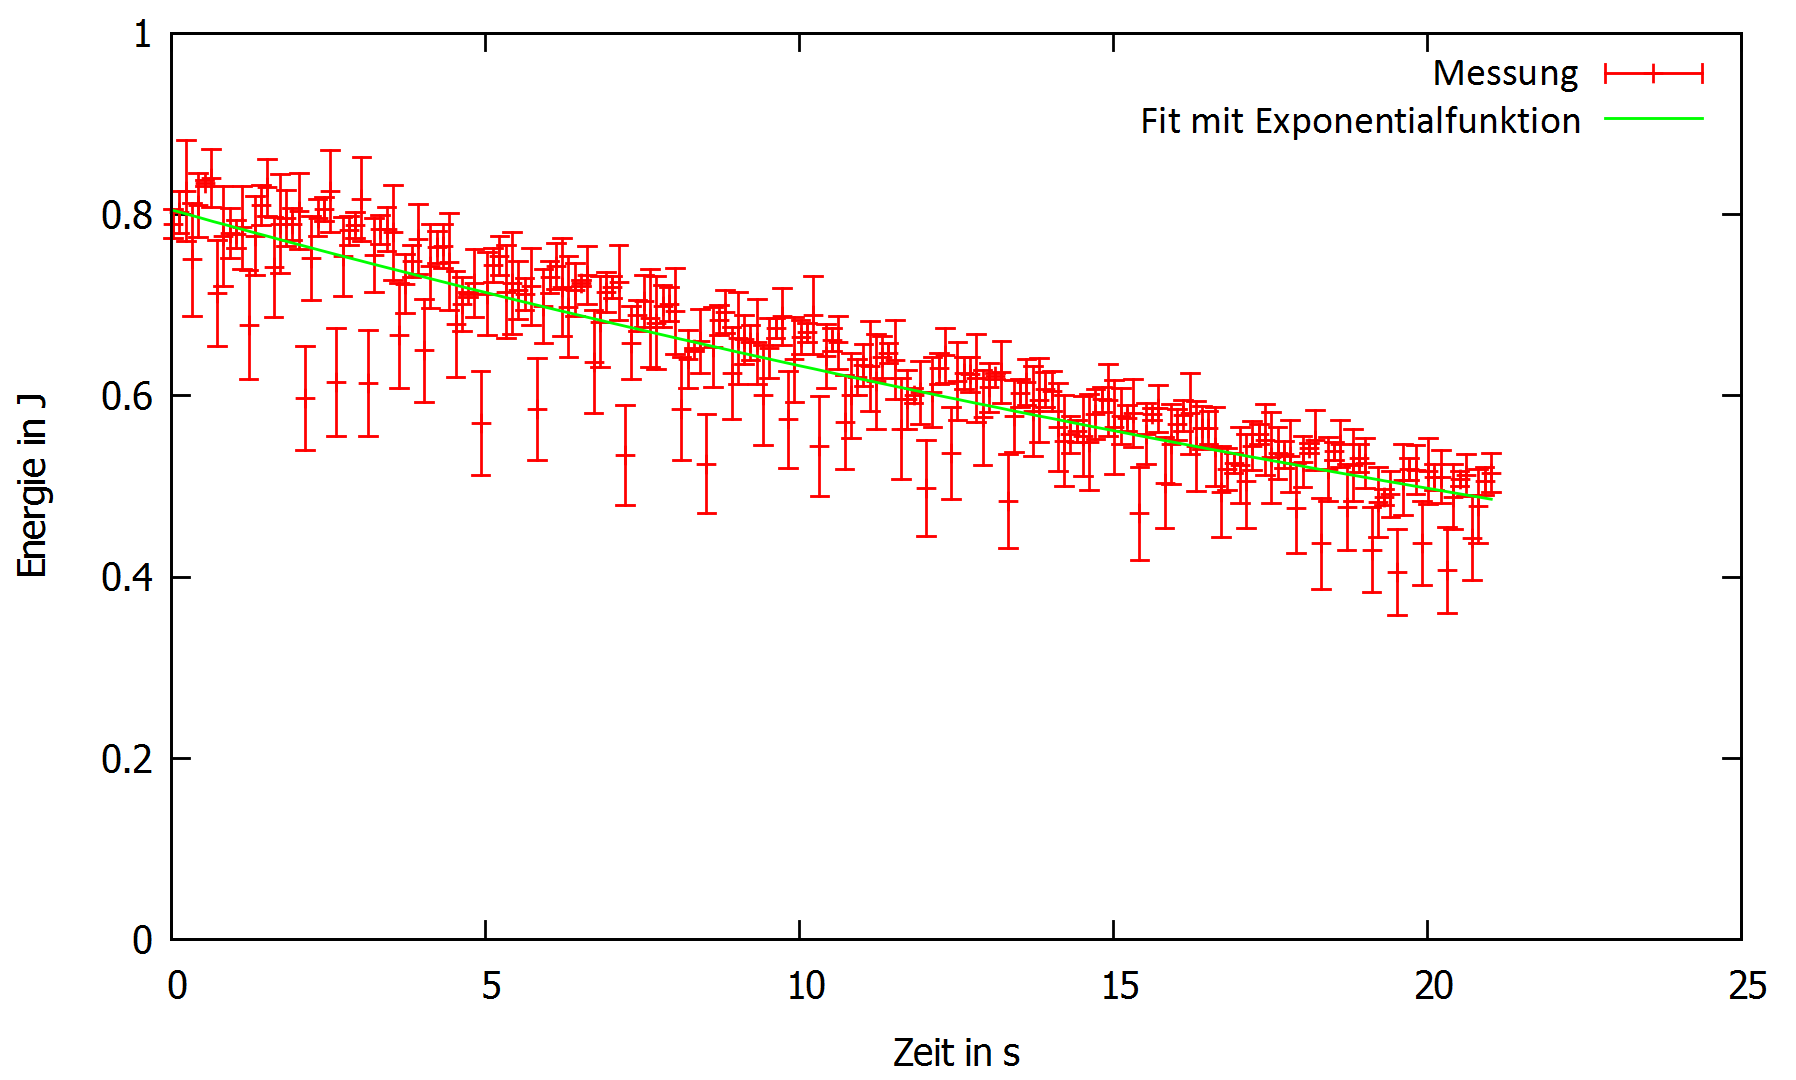
\includegraphics[width=.9\textwidth]{images/E_ueber_t_neu.png}
\caption{Energie des Pendels über der Zeit}
\label{E_ueber_t}
\end{figure}
In Abb. \ref{E_ueber_t} wurde die Gesamtenergie des Pendels über der Zeit aufgetragen. Die Energie wurde dabei nach 
\begin{equation}
E(t) = E_{kin,1}(t) + E_{kin,2}(t) + E_{pot,1}(t) + E_{pot,2}(t) = \frac{1}{2} (m_1 \cdot \vec{v_1}(t)^2 + m_2 \cdot \vec{v_2}(t)^2) + g (m_1 \cdot h_1(t) + m_2 \cdot h_2(t))
\end{equation}
berechnet, wobei $h_1 = y_1 + l_1$ und $h_2 = y_2 + l_1 + l_2$, sodass $h_1 $ und $h_2$ die Höhe über der Ruhelage des entsprechenden Pendels angeben. 
Somit ist die Energie im Fall, dass sich das Pendel gänzlich in Ruhe und in der Ruhelage ($phi_1, phi_2 = 0$) befindet, auf 0 normiert. 
Zunächst fällt auf, dass die Energiewerte (Abb. \ref{E_ueber_t}) deutlich streuen und vom einem montonen Verlauf abweichen. Der Grund hierfür besteht darin, dass das ausgewertete Video lediglich mit einer Aufnahmerate von 30 Bildern pro Sekunde aufgezeichnet wurde. Aus diesem Grund tritt der Effekt auf, dass die Spitzen der Geschwindigkeit bei der Auswertung \enquote{abgeflacht} werden. Dies ist insbesondere dann sichtbar, wenn das Pendel ein Minimum der Höhe durchläuft und ein Bild vor und das darauffolgende nach dem Durchlauf aufgenommen wird. Die errechnete Geschwindigkeit ist dann kleiner als die tatsächliche (Abb. \ref{grafik1}). 

\begin{figure}
        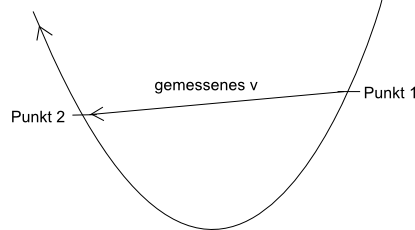
\includegraphics[width=.7\textwidth]{images/grafik1.png}
\caption{Schematische Darstellung der fehlerhaften Auswertung}
\label{grafik1}
\end{figure}

Dieser durch die Aufnahmerate von 30 Bildern pro Sekunde bedingte Fehler ist schwer zu quantifizieren. Um in etwa die Größenordnung 
des Fehlers abzuschätzen, soll folgende Abschätzung betrachtet werden: 
Aus Abb. \ref{v_ueber_t} geht hervor, dass die obere Masse maximal eine Geschwindigkeit von etwa $1.8 \frac{m}{s} $ hat. Nimmt man an, 
dass sich diese Masse auf einer Kreisbahn und mit etwa dieser Geschwindigkeit für $\frac{2}{30} s$ bewegt, so kann der in 
Abb. \ref{graphik1} dargestellte Fehler für diese Idealisierung berechnet werden: 
Aus $ v = 1.8 \frac{m}{s} $ ergibt sich mit $ l_1 = 0.2 m$ eine Winkelgeschwindigkeit von $ \omega = 9 \frac{1}{s} $. Für die Dauer
einer Belichtungszeit beträgt der Winkel, um den sich das Pendel also bewegt, etwa $ \Delta \phi = \omega \cdot \Delta t = 9 \frac{1}{s} \cdot \frac{1}{30} s = 0.3$. 
Da für die Geschwindigkeitsberechnung zwei Belichtungsintervalle betrachtet werden, ergibt sich aus Abb. \ref{graphik1} und elementarer 
Geometrie, dass das Verhältnis zwischen tatsächlich zurückgelegter Strecke und der verkürzten Strecke, aus der in der Auswertung die Geschwindigkeit bestimmt 
wird, sich zu $ \frac{2 \Delta \phi \cdot l_1}{2 \cdot \sin(\Delta \phi) \cdot l_1} = \frac{\Delta \phi}{\sin(\Delta \phi)} $
ergibt. Für ein $\Delta \phi $ von 0.3 ergibt sich ein Verhältnis von $1.015$, was also $1.5 \% $ Abweichung entspricht. 
Da hier maximale Werte verwendet wurden, ist dies ebenfalls der maximale Fehler, der sich aus dem erklärten Effekt ergeben sollte. 
Mittels einer Fehlerfortpflanzung ergibt sich: 

\begin{align}
\Delta E &= \sqrt{(\frac{\partial E}{\partial v_1} \cdot \Delta v_1)^2 + (\frac{\partial E}{\partial v_2} \cdot \Delta v_2)^2} = \sqrt{(m_1 |v_1| \cdot \Delta v_1)^2 + (m_2 |v_2| \cdot \Delta v_2)^2}= \nonumber \\ &= \sqrt{(\Delta v)^2 \cdot (m_1^2 |v_1|^2 + m_2^2 |v_2|^2)}, 
\end{align}
wobei $ \Delta v_1 = \Delta v_2 = \Delta v  = 0.03$. 
Damit ergeben sich die eingezeichneten Fehlerbalken. 


\begin{figure}
        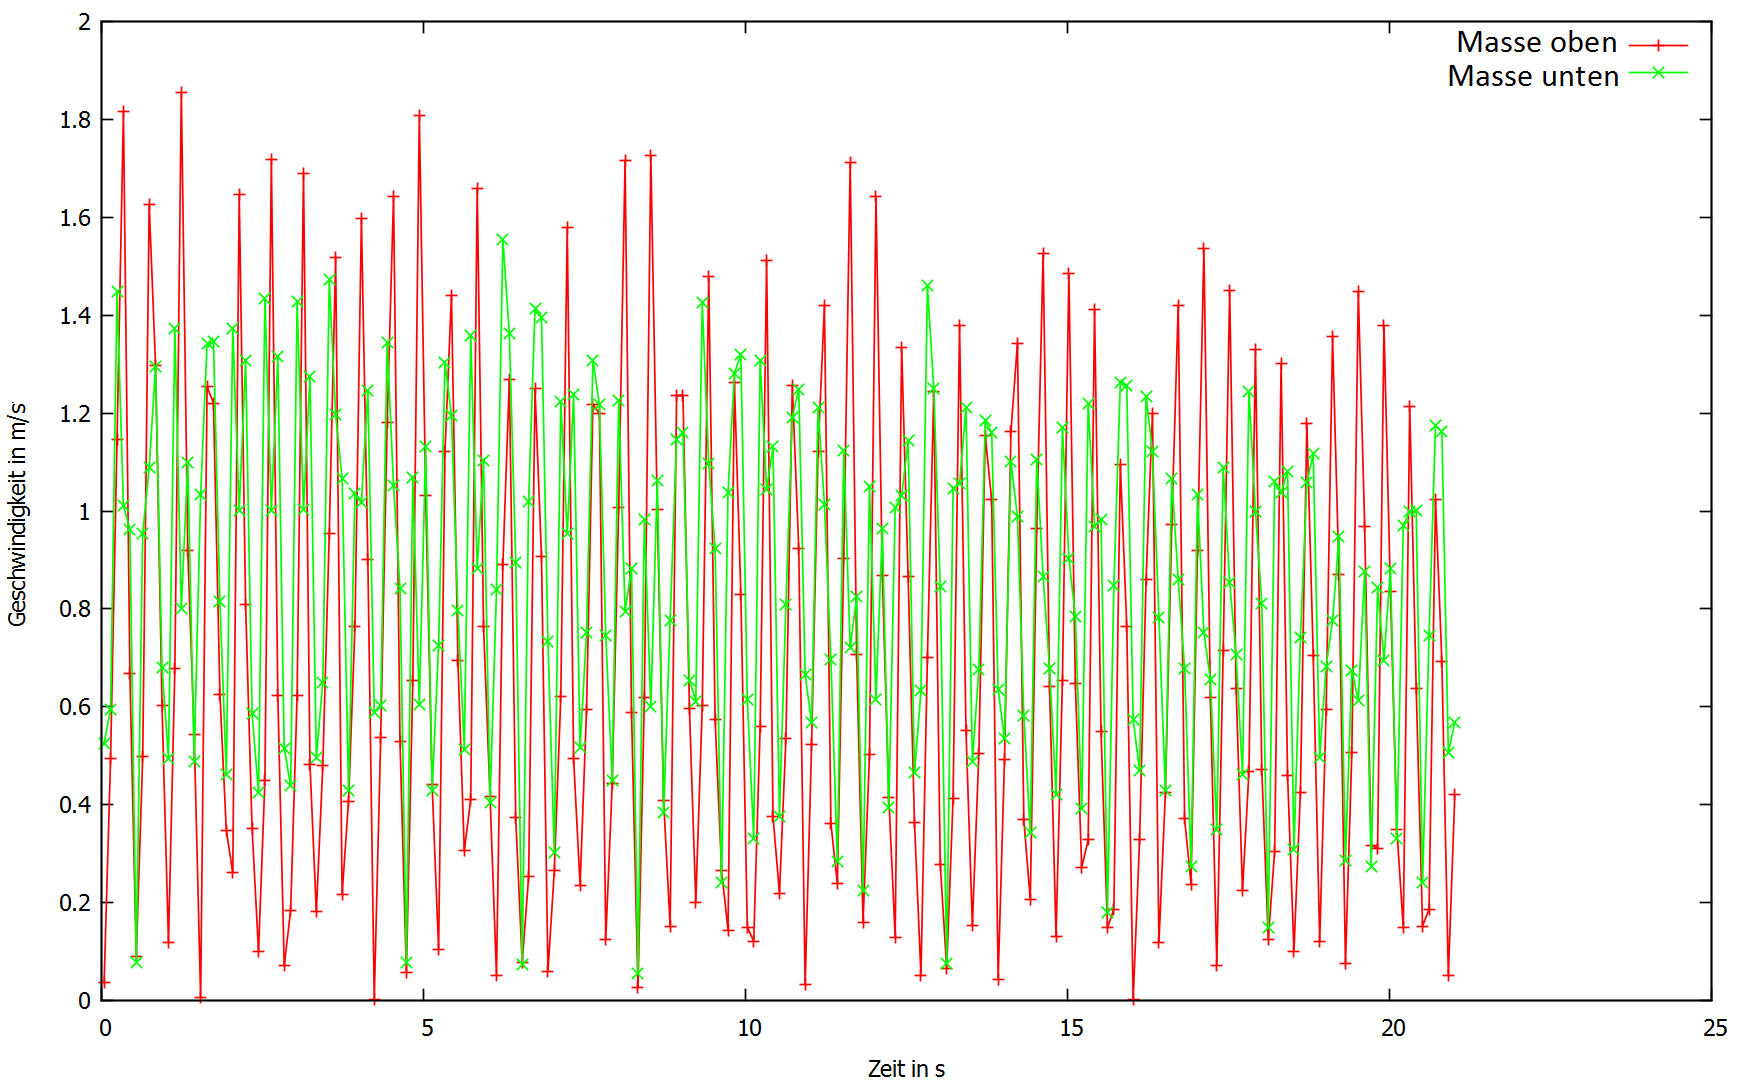
\includegraphics[width=.9\textwidth]{images/v_ueber_t_neu.png}
\caption{Geschwindigkeit der beiden Massepunkte über der Zeit}
\label{v_ueber_t}
\end{figure}


\subsubsection{Luftreibung}
Da sich die Geschwindigkeit im Bereich von etwa null bis zwei Metern pro Sekunde bewegt, siehe Abb. \ref{v_ueber_t}, eine der verwendeten Acrylplatten eine Projektionsfläche von $ 1.5 \cdot 10^{-3} m^2$ (unten: 25 cm Länge, 6 mm Stärke) bzw. $ 1.4 \cdot 10^{-3} m^2$ (oben: 35 cm Länge, 4 mm Stärke) hat, ergibt sich bei einer Luftdichte von $ 1.2 \frac{kg}{m^2} $ eine abbremsende Kraft von $ 1.8 \cdot 10^{-3} N $ (mit $ v = 1 \frac{m}{s}, c_W = 2, A_S = 1.5 \cdot 10^{-3} m^2 $). 

Für die drei verwendeten Platten ergibt sich somit, mit der stark vereinfachten Annahme, dass die gesamte Fläche sich mit gleicher Geschwindigkeit bewegt und die Beschleunigung über längere Zeit konstant ist, was zur Abschätzung der Größenordnung aber ausreichend ist, eine Kraft von $ 5.4 \cdot 10^{-3}  N $. Mit einer Gesamtmasse von $0.7 kg$ inklusive der Acrylplatten folgt eine durchschnittliche Beschleunigung von etwa $ 7.7 \cdot 10^{-3} \frac{m}{s^2} $. Bei einer Dauer der Messung von $20 s$ ergibt sich hiermit also  eine Geschwindigkeitsänderung von etwa $ 0.15 \frac{m}{s} $, die also einen wesentlichen Teil des Energieverlusts darstellt. \\
\begin{comment}
Die Luftreibung soll qualitativ für ein einfaches Pendel diskutiert werden: Die Reibungskraft selbst ist nach (\ref{luftreibung}) proportional zu $v^2$. Für den Energieverlust $\frac{dE}{dt}$ gilt:
\begin{equation}
\frac{d E}{d t} = \frac{\vec{F} \cdot d\vec{s}}{dt} \sim  \vec{F} \cdot \vec{v} \sim |v|^3, 
\end{equation}
da Kraft und Geschwindigkeit im Fall des einfachen Pendels in die gleiche Richtung zeigen. 
Der Energieverlust wird nun über eine Schwingung integriert, was mit $ v(t) = v_0 \cdot \sin(\frac{2 \pi t}{T})$:
\begin{equation}
\int _0^{2\pi} |v|^3 dt = \int _0^{2\pi}( v_0^3 \cdot |\sin(\frac{2 \pi t}{T})^3|)dt = v_0^3 \cdot c,
\end{equation}
wobei $ c = \int _0^{2\pi} |\sin(\frac{2 \pi t}{T})^3|dt $ eine hier nicht näher bestimmte Konstante. 
Da die Energie eines Pendels proportional zum Quadrat der Maximalgeschwindigkeit ist, ergibt sich für den Energieverlauf folgende Differentialgleichung: 
\begin{equation}
\frac{dE}{dt} \sim v^3 \sim E^{1.5}. 
\end{equation}
Die allgemeine Lösung dieser Gleichung ist: 
\begin{equation}
E(t) = a \cdot (bt + d)^{-2}. 
\end{equation}
Dieses Ergebnis ist allerdings nur bedingt auf ein Doppelpendel übertragbar, da dort die Geschwindigkeit nicht einer einfachen Sinus-Funktion folgt. 
\end{comment}
\subsubsection{Reibung in den Kugellagern}
Laut \cite{wiki} liegt $ c_R $ für Kugellager im Bereich von etwa 
$ 0.5 $ bis $ 1 \cdot 10^{-3} $. 
Damit ergäbe sich bei einer Gesamtmasse von etwa $ 0.7 \  kg  $ eine abbremsende Kraft von der Größenordnung $ 10^{-3} $ bis $ 10^{-2} N $. 

\subsubsection{Energieübertrag auf die Aufhängung}
Neben dem Energieverlust durch die Luftreibung tritt ein der Energieübertrag auf die Aufhängung als weiterer Effekt auf. Dieser sollte zwar durch eine möglichst starre und unbewegliche Befestigung des Pendels zwischen zwei Tischen minimiert werden, trotzdem fangen vor allem bei Überschlägen des Pendels die Tische deutlich sichtbar zu wackeln an. 
Es bietet sich hier an, in grober Näherung eine lineare Abhängigkeit des Energieverlustes des Systems von der momentanen Energie anzunehmen. 

Nimmt man einen exponentiellen Abfall der Energie $ E(t) = a \cdot e^{b \cdot t} $ an, so ergibt sich mittels eines Fits (Abb. \ref{E_ueber_t}) in den Verlauf von 

\begin{equation}
 a = 0.813   J
\nonumber
\end{equation}  und  
\begin{equation}
b = -0.024  s^{-1}
\nonumber
\end{equation} 
mit Fehlern von $1.26 \% $ und $ 4.89 \% $. \\
Allerdings kann aus den hier dargestellten Daten nicht verifiziert werden, ob der Verlauf tatsächlich einem exponentiellen Abfall folgt, da auch etwa ein Abfall mit dem inversen Quadrat der Zeit denkbar wäre, wie es für reine Luftreibung zu erwarten wäre. 

\subsection{Simulation des Doppelpendels}
Die gemessenen Daten sollen nun mit einer Simulation, die entsprechend der Beschreibung in der Theorie durchgeführt wurde, verglichen werden. Da das Pendel händisch gestartet wurde, ist davon auszugehen, dass sich die ersten Werte eher schlecht mit der Simulation nachvollziehen lassen. 


\begin{figure}
        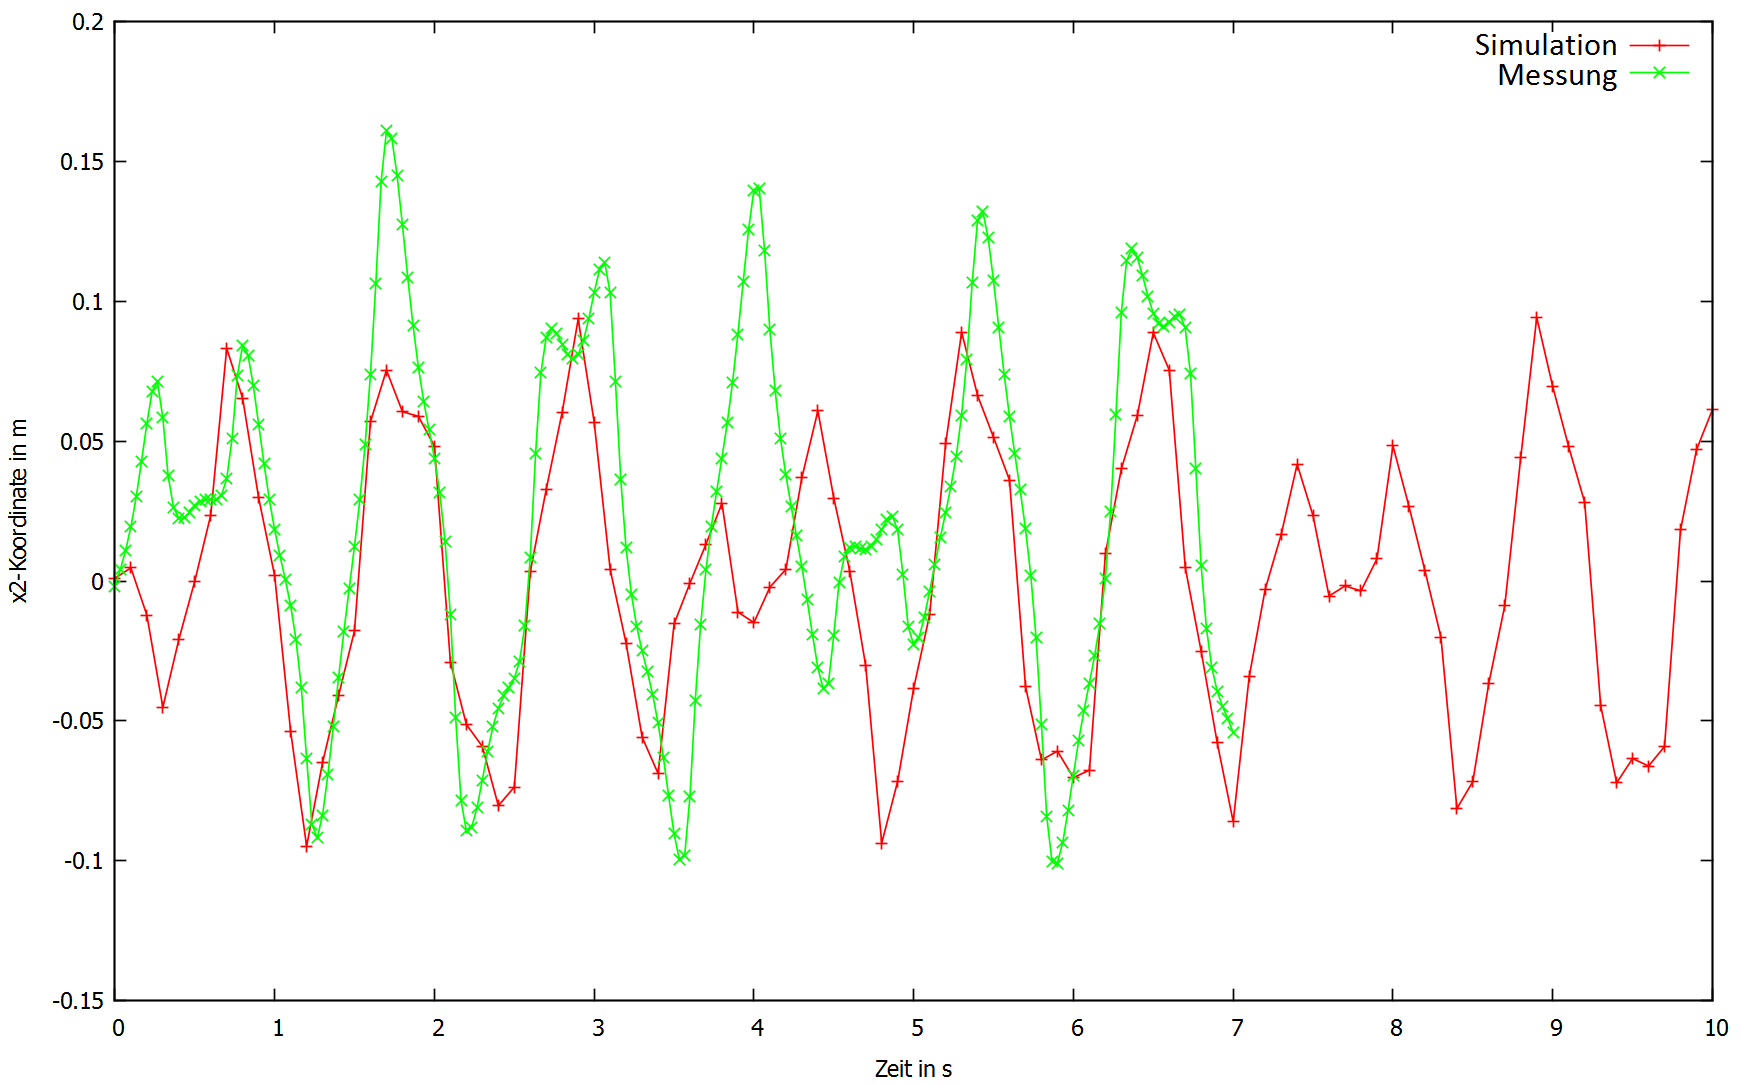
\includegraphics[width=.9\textwidth]{images/x2_ueber_t_beginn_neu.png}
\caption{Auftragung der $x_2$-Koordiante bei einer Simulation mit Start zu etwa dem Zeitpunkt des Loslassens}
\label{x2_ueber_t_alt}
\end{figure}


Tatsächlich ist dies der Fall, wie in Abb. \ref{x2_ueber_t_alt} zu sehen ist. Hier ist die $x_2$-Koordinate, also die x-Koordinate des unteren Pendels über der Zeit aufgetragen. Man erkennt, dass sich Simulation und Messung schon zu Beginn sehr deutlich unterscheiden. Zwar verlaufen ab etwa $ 0.8 s $ Simulation und Messung ähnlich, allerdings dürfte dies auf einen Zufall beziehungsweise darauf zurückzuführen sein, dass die Auslenkung des Pendels hier relativ klein ist und das Pendel ein leicht peroidisches Verhalten aufweist. 
Aus diesem Grund wurde die Simulation erst bei $ 0.8 s $ begonnen. Dieser spezielle Wert wurde gewählt, weil hier wie in \aref{x2_ueber_t_alt} die Änderungsrate von $x_2$ in etwa 0 ist, und so Fehler bei der Bestimmung der Geschwindigkeit zu minimieren. 

\begin{figure}
        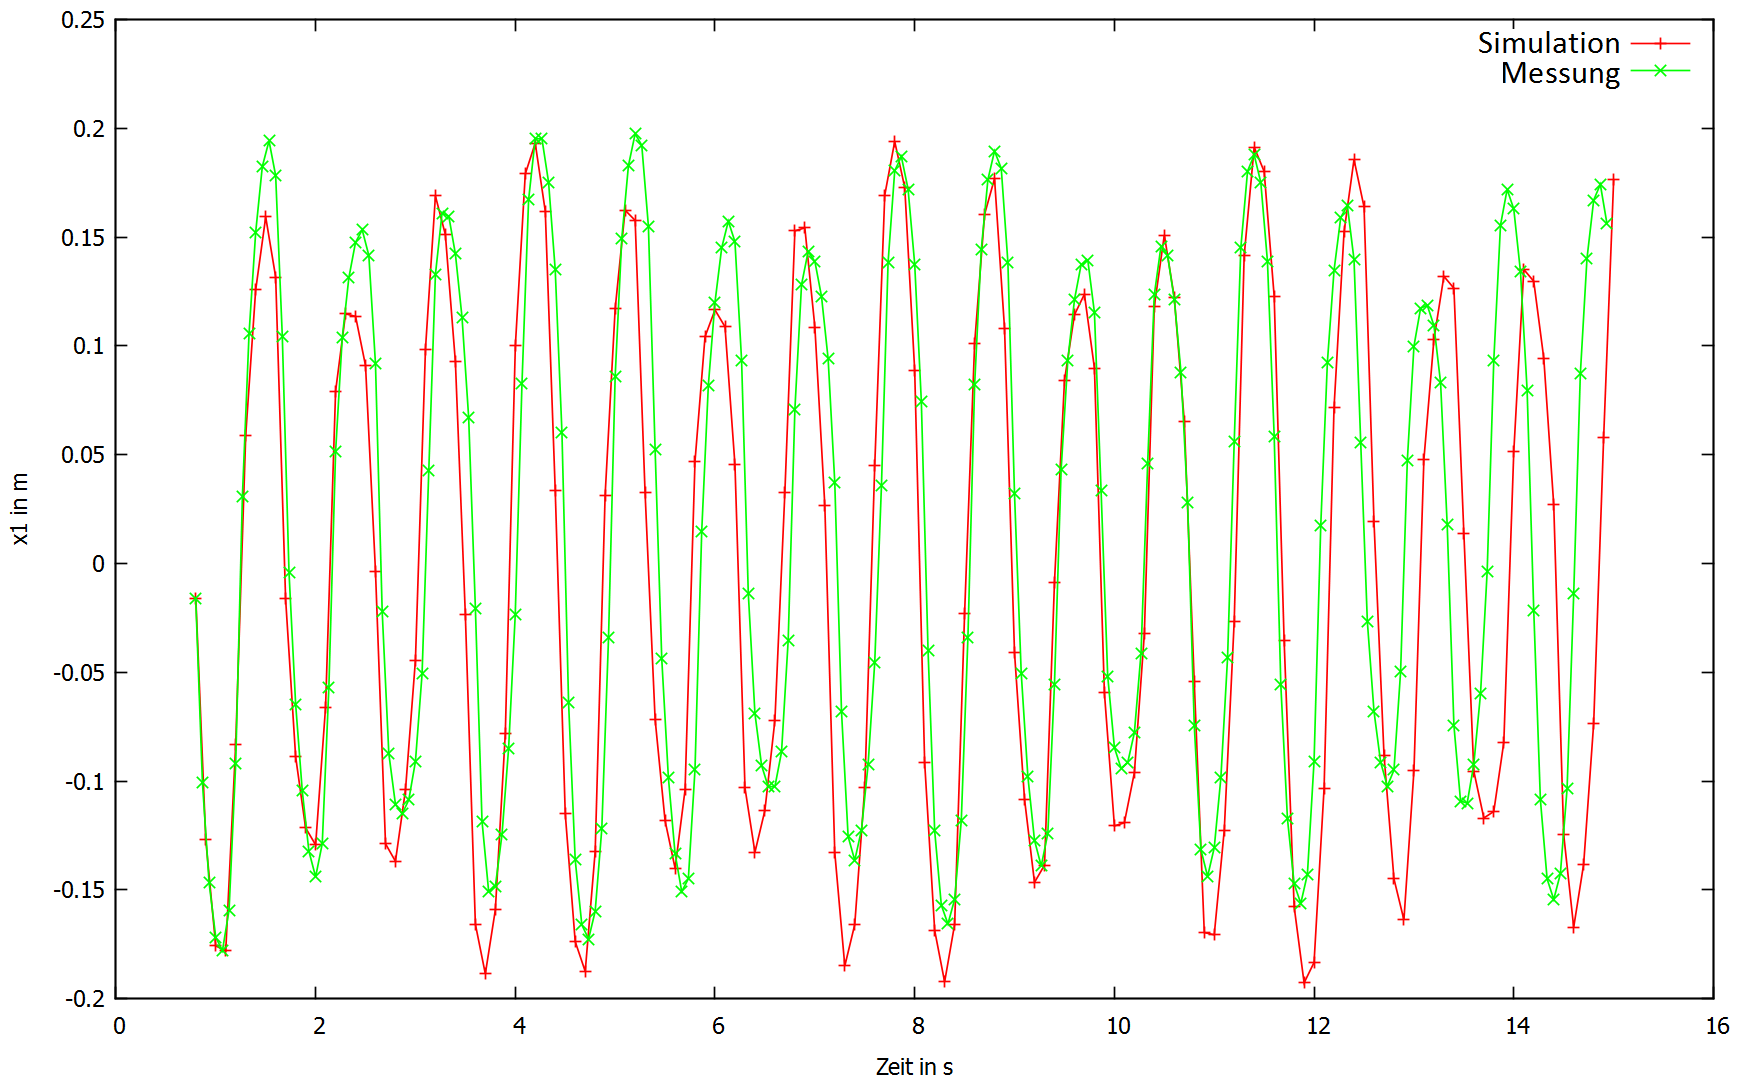
\includegraphics[width=.9\textwidth]{images/x1_ueber_t_neu.png}
\caption{Auftragung der $x_1$-Koordiante bei einer Simulation mit späterem Start}
\label{x1_ueber_t}
\end{figure}

\begin{figure}
        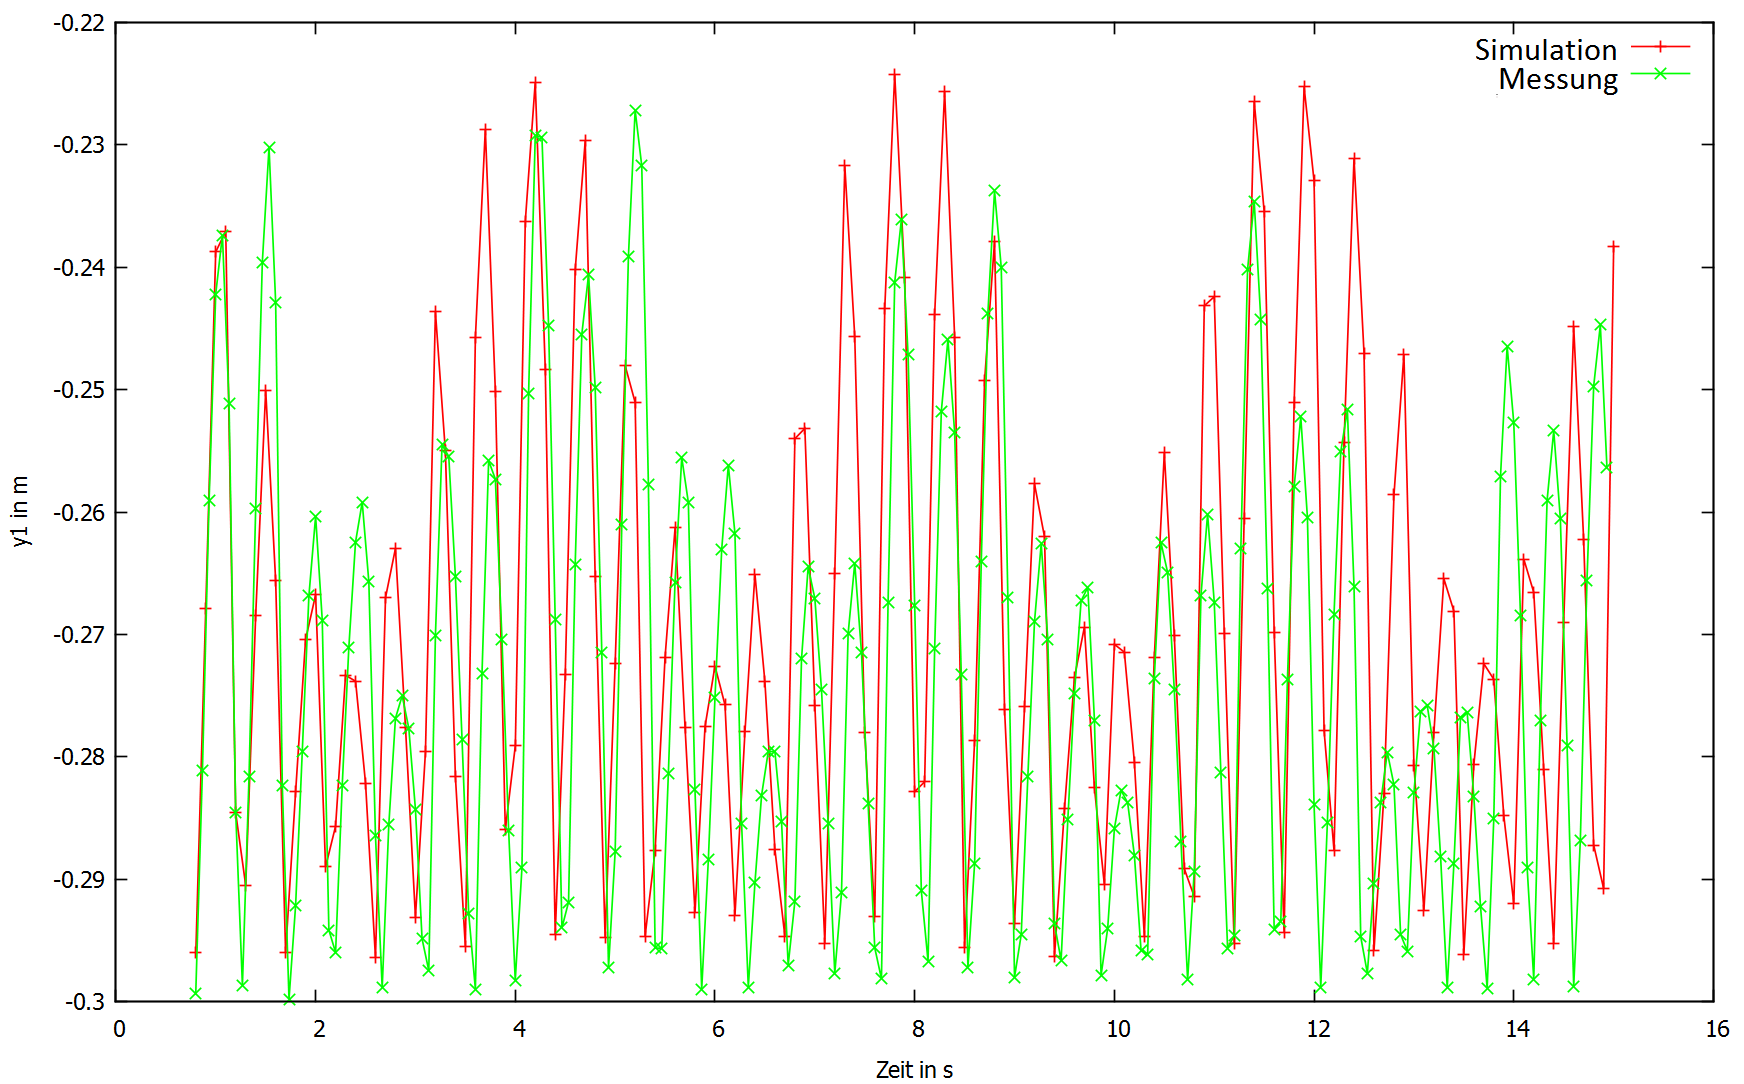
\includegraphics[width=.9\textwidth]{images/y1_ueber_t_neu.png}
\caption{Auftragung der $y_1$-Koordiante bei einer Simulation mit späterem Start}
\label{y1_ueber_t}
\end{figure}

\begin{figure}
        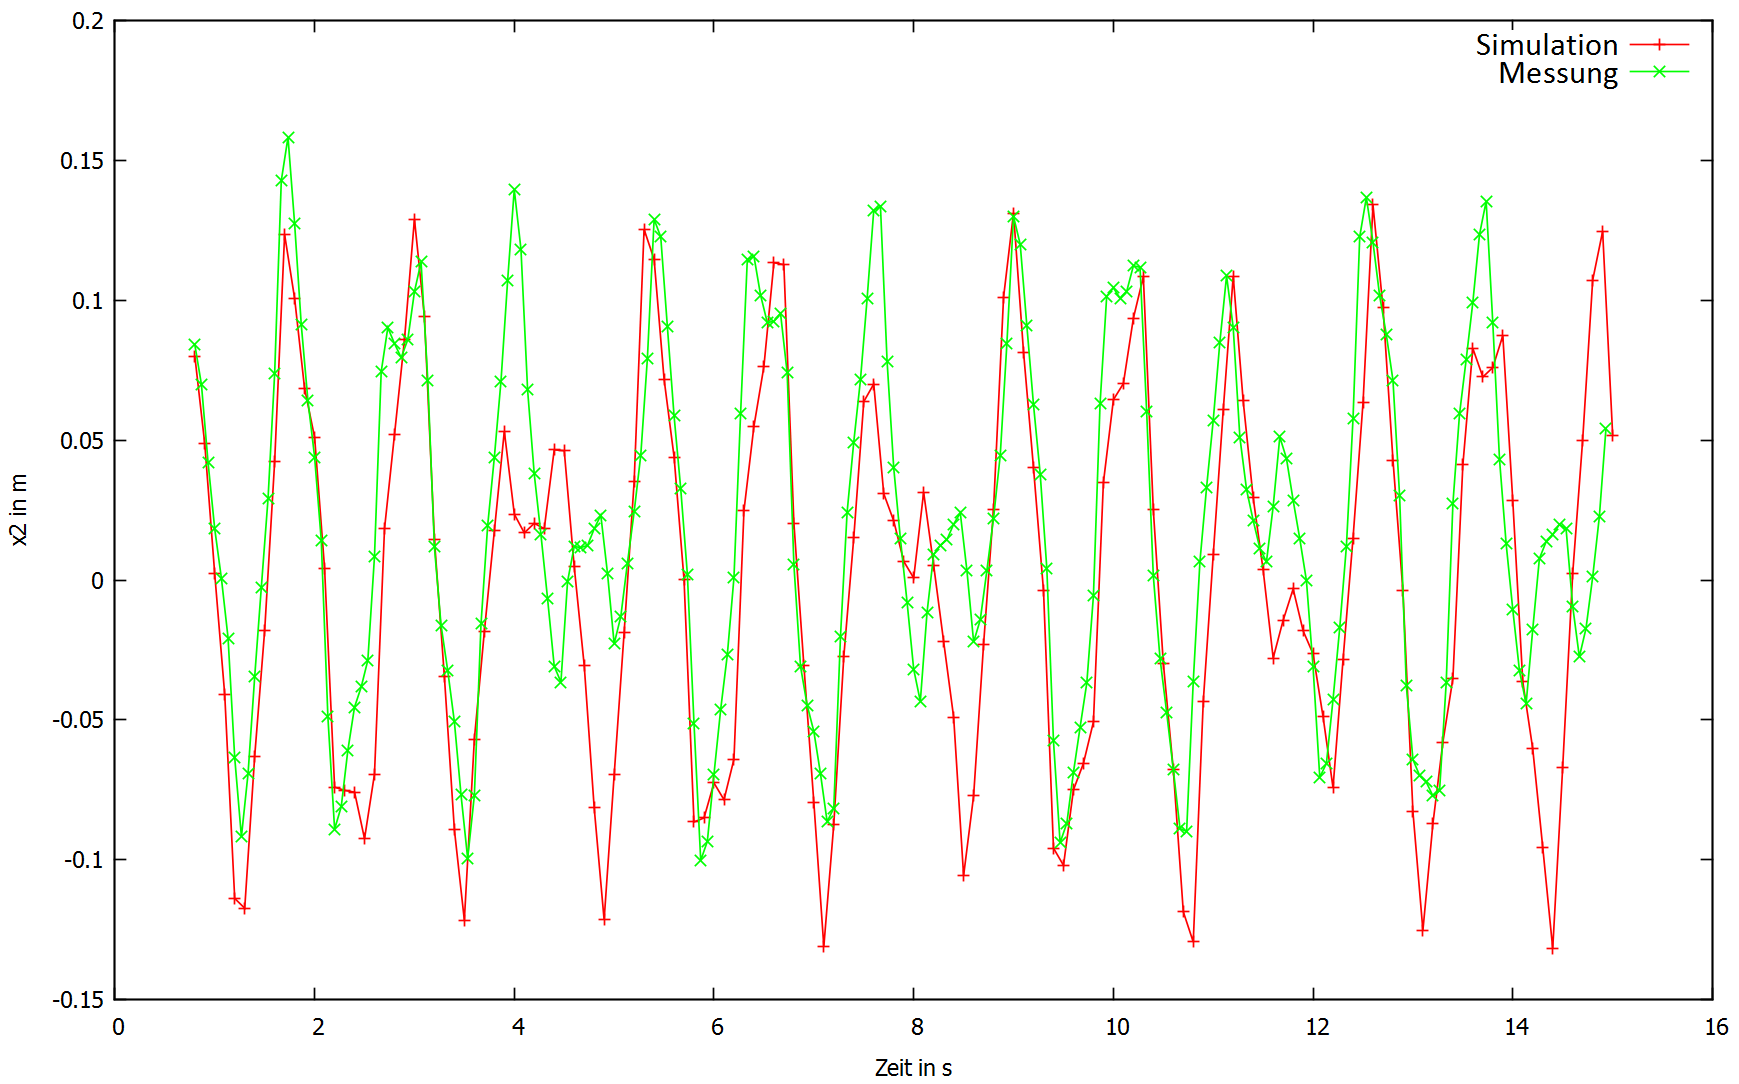
\includegraphics[width=.9\textwidth]{images/x2_ueber_t_neu.png}
\caption{Auftragung der $x_2$-Koordiante bei einer Simulation mit späterem Start}
\label{x2_ueber_t}
\end{figure}

\begin{figure}
        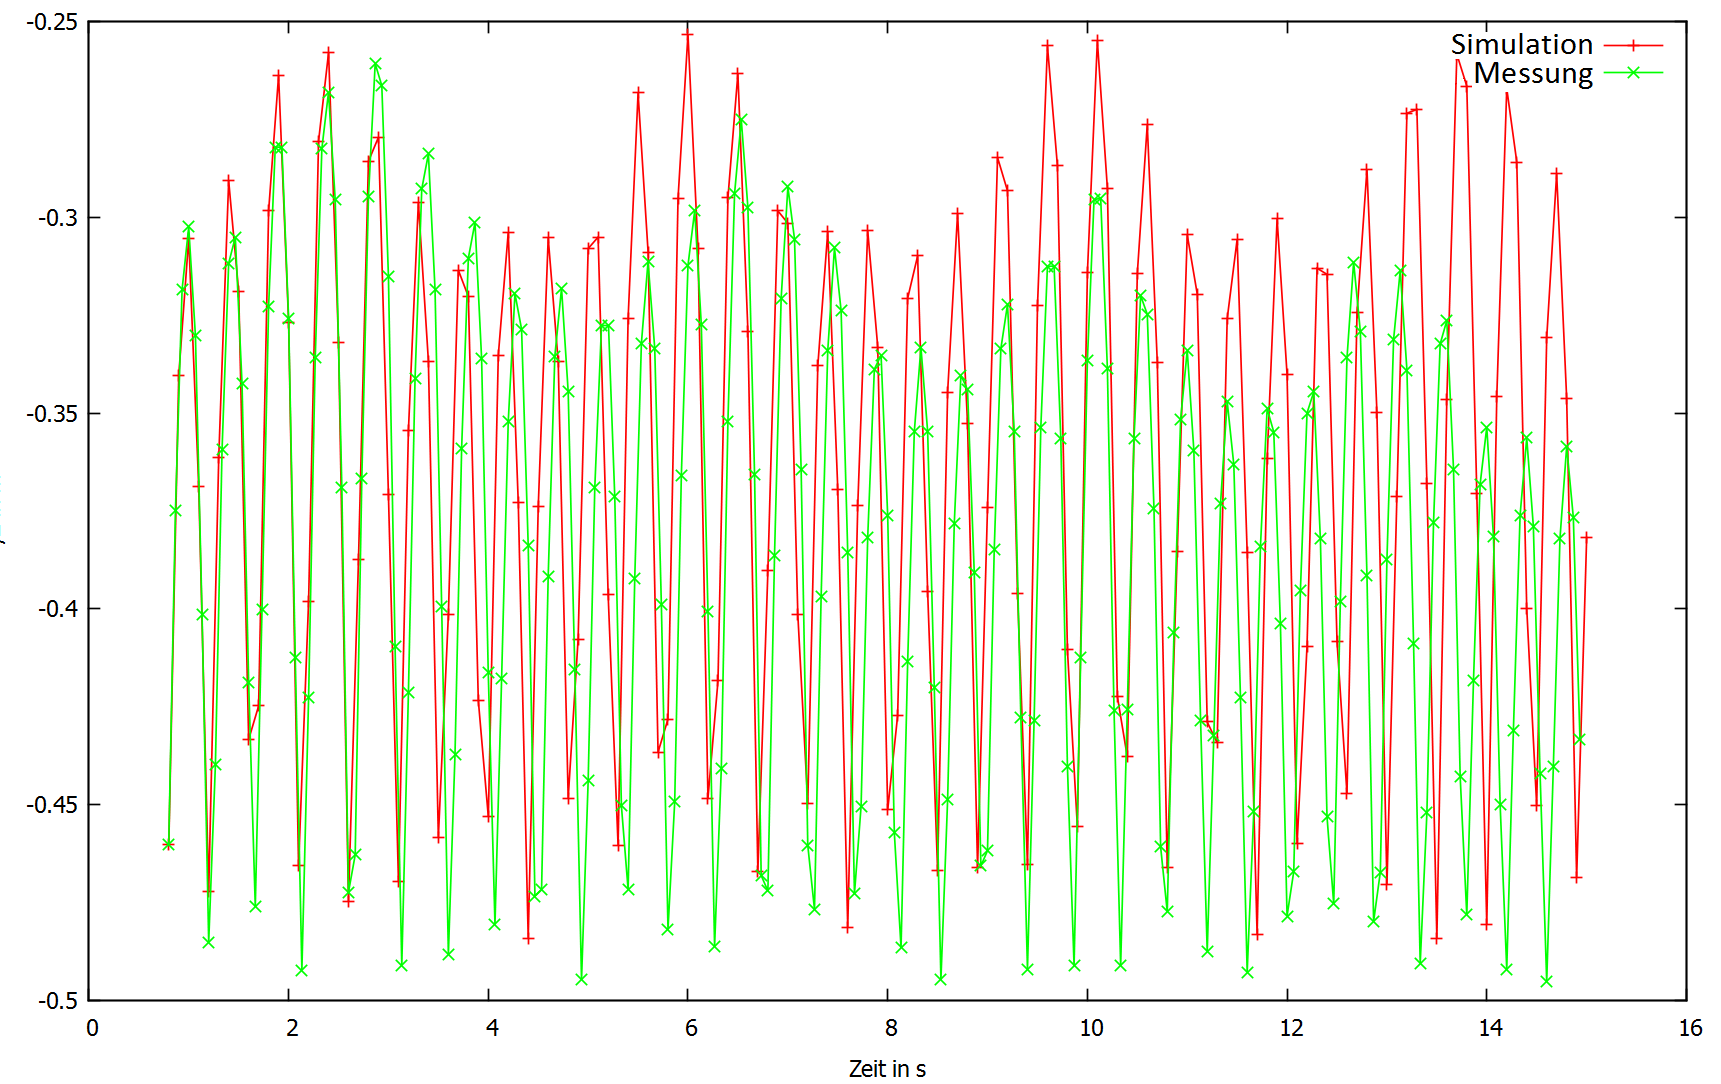
\includegraphics[width=.9\textwidth]{images/y2_ueber_t_neu.png}
\caption{Auftragung der $y_2$-Koordiante bei einer Simulation mit späterem Start}
\label{y2_ueber_t}
\end{figure}

Dabei wurden die in Abb. \ref{x1_ueber_t}, \ref{y1_ueber_t}, \ref{x2_ueber_t} und Abb. \ref{y2_ueber_t} dargestellten Ergebnisse erzielt, wobei der rote Graph die Simulation darstellt und der grüne die tatsächlich gemessenen Werte. \\
Es ist deutlich sichtbar, dass die Verläufe bis etwa $ t = 2 s $ recht gut mit den Messwerten übereinstimmen, danach ergeben sich vor allem bei den $x_2- $ und $ y_1$-Koordinaten deutliche Unterschiede, wohingegen bei den anderen beiden Koordinaten noch länger eine deutliche Ähnlichkeit bestehen bleibt. Die Ähnlichkeit ist zum Teil auch darauf zurückzuführen, dass das Pendel bei dieser Messung kein deutlich ausgeprägtes chaotisches Verhalten besitzt, sondern eher periodische Eigenschaften aufweist. \\
Trotzdem eignet sich die Simulation scheinbar gut, um die Bewegung des Pendels nachzuvollziehen. 

\begin{figure}
        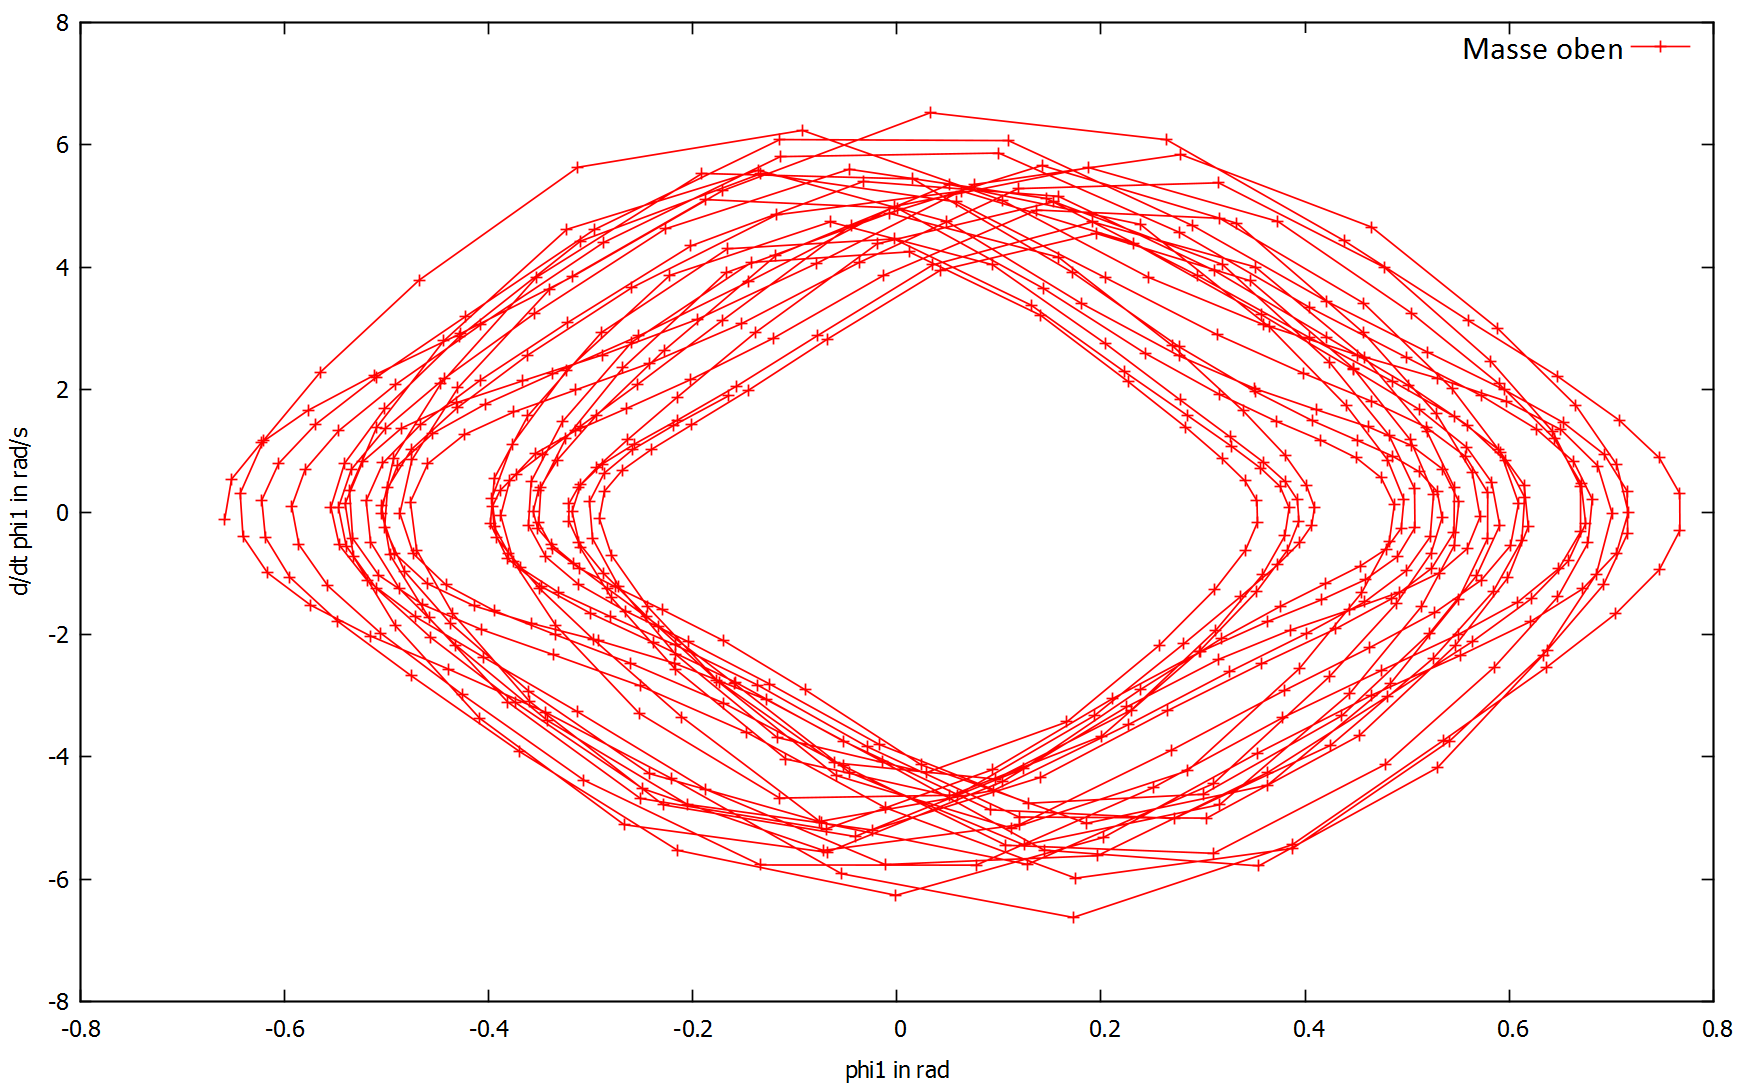
\includegraphics[width=.9\textwidth]{images/phi1_ueberphi1_neu.png}
\caption{Phasenraum $\dot{\varphi_1} $ über $\varphi_1$}
\label{phi1}
\end{figure}

\begin{figure}
        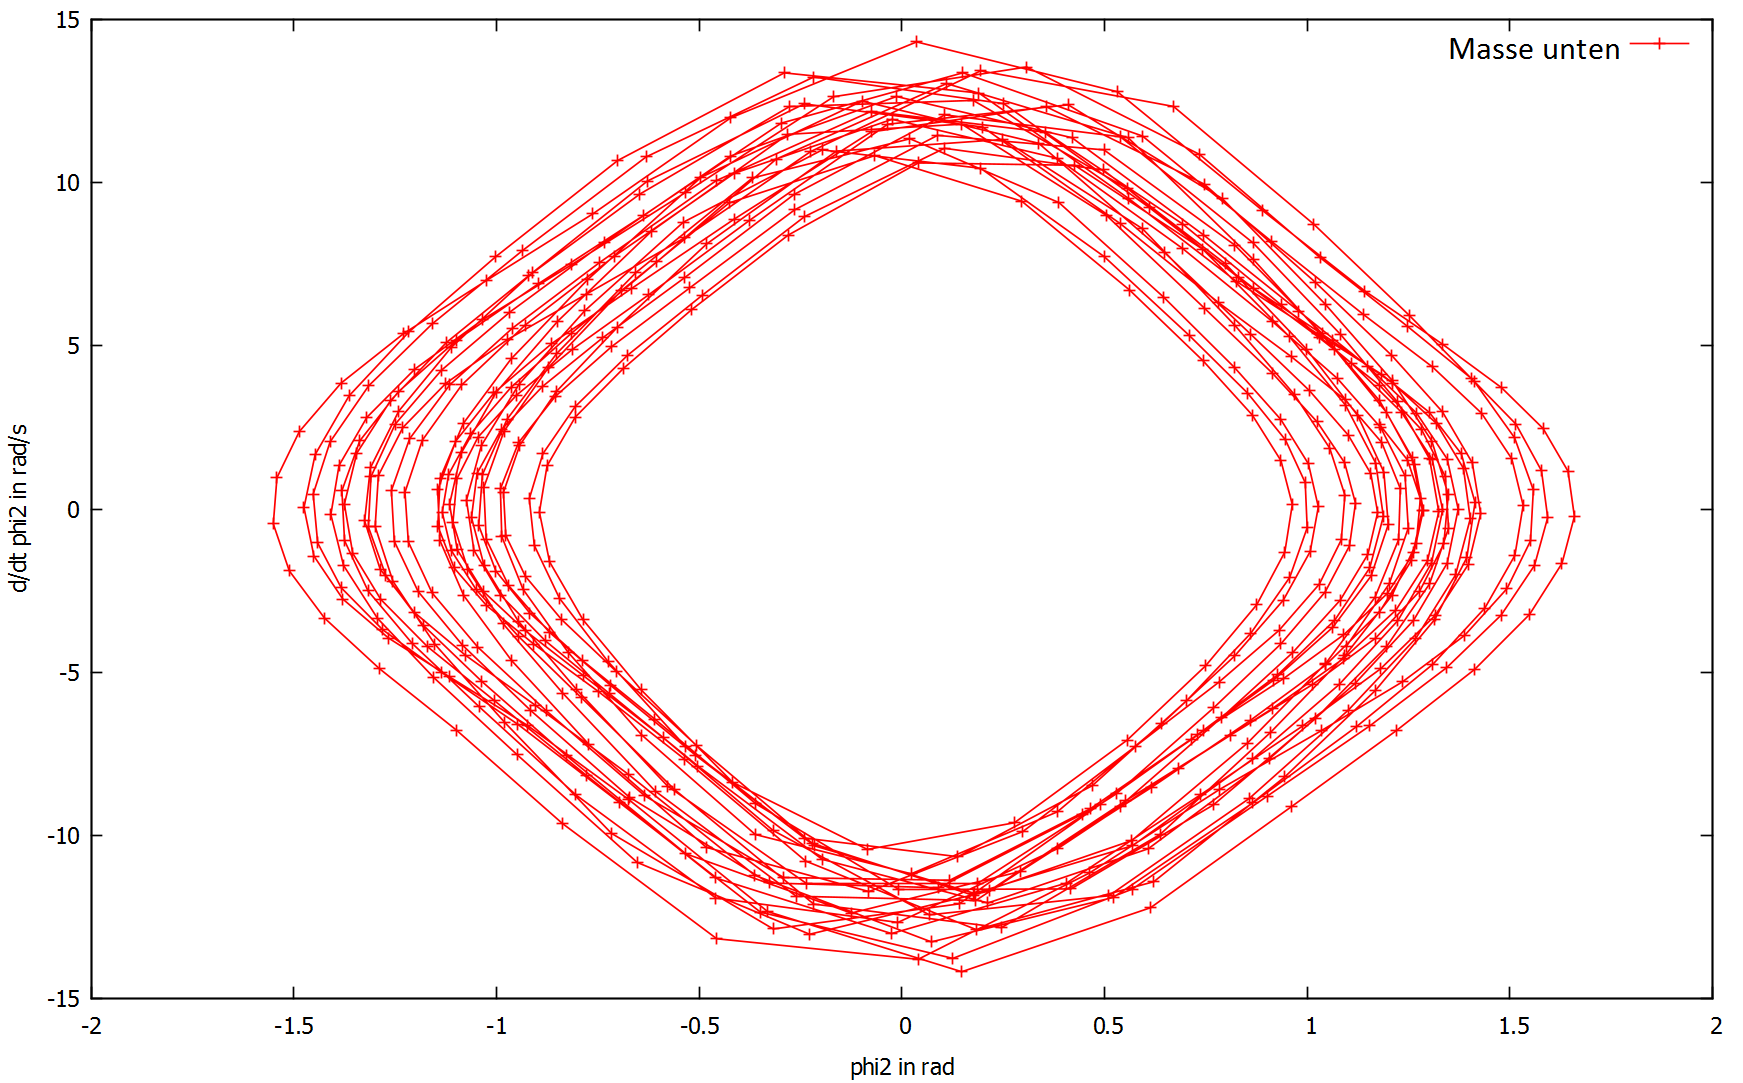
\includegraphics[width=.9\textwidth]{images/phi2_ueberphi2_neu.png}
\caption{Phasenraum $\dot{\varphi_2} $ über $\varphi_2$}
\label{phi2}
\end{figure}

Weiter sind die sich aus den gemessenen Daten ergebenden Phasenraumdiagramme in Abb. \ref{phi1} und Abb. \ref{phi2} dargestellt. Es ergibt sich dabei ein Verlauf, der plausibel erscheint, da sie sehr dem in Abb. \ref{pic:pendel_einfach} ähnelt, welches das Phasenraumdiagramm eines einfachen Pendels zeigt. Der Grund dafür liegt darin, dass auch das Doppelpendel in dem hier dargestellten Energiebereich leldiglich \enquote{hin und her schwingt}, sodass eine in Näherung ellipsenförmige, auf jeden Fall aber \enquote{geschlossene} Kurve entsteht. \\
Trotzdem gibt es Abweichungen zum einfachen Pendel. Zunächst schneiden sich hier die Linien im Phasenraumdiagramm, was allerdings darauf zurückzuführen ist, dass die Auftragungen nur eine Projektion des gesamten, vierdimensionalen Phasenraums darstellen. Weiter erscheint das Diagramm vor allem bei dem oberen Pendel (\aref{phi1}) seitlich \enquote{unscharf}, was durch die Beeinflussung durch das untere Pendel zu erklären ist. 

\section{Fazit}
Es zeigt sich, dass das Doppelpendel, wie zu erwarten, chaotisches Verhalten aufweist. Darüber hinaus ist es möglich, die Bewegung des Doppelpendels über mehrere \enquote{Schwingungen} nachzuvollziehen, wohingegen eine analytische Lösung der in der Theorie aufgestellten Bewegungsgleichung unmöglich ist. 
